\chapter{Erweiterung des Werkzeugkastens: Bauteilkunde}

Nach Erarbeitung der bisherigen Kapitel sind nun die wichtigsten Grundlagen zum Arduino gelegt. Die folgenden Seiten bieten jeweils eine Einführung in neue Bauteile, für die unterschiedliche Grundlagen aus den bisherigen Kapiteln benötigt werden. Dazu waren bisher jeweils Hinweise mit Links zu den entsprechenden Abschnitten eingestreut, ab wann die nötigen Grundlagen für die Bauteile und deren Projekte gelegt waren. Daher finden sich neben den Bauteilen in den folgenden Abschnitten jeweils Links, die an die entsprechenden Stellen im Skript zurückführen und auch zur Wiederholung der Grundlagen dienen können.

\medskip
\begin{ziel}
	Überlegt euch zu zweit ein Arduino-Projekt, das ihr gerne umsetzen würdet, und erarbeitet euch die fehlenden Grundlagen dazu. Ihr könnt alle Bauteile aus eurem Arduino-Kit nutzen. Die folgenden Abschnitte geben euch eine Einführung zu den einigen Bauteilen und ggf. bieten sie euch auch Ideen, was man mit dem Arduino umsetzen kann.
	
	Am Ende solltet ihr euer Projekt mit einem funktionierenden Prototypen auf einem Steckbrett vorstellen können. Zudem sollt ihr eine kurze Ausarbeitung mit folgenden Abschnitten anfertigen:
	\begin{multicols}{2}
		\begin{itemize}[parsep=0mm, itemsep=0ex]
			\item Projektziel
			\item Materialliste
			\item Schaltplan
			\item Programm (als Screenshot)
			\item Erläuterung des Schaltplans und des Programms
			\item Ausblick: Mögliche Erweiterungen oder Anwendungen
		\end{itemize}
	\end{multicols}
\end{ziel}

\bigskip

\begin{projektueberblick}
	\item Alarmanlage \dotfill \pageref{proj:neigungsalarmanlage}
	\item Carport-Lampe \dotfill \pageref{proj:carport}
	\item Einparkhilfe für ein Auto \dotfill \pageref{proj:einparkhilfe}
	\item Uhr \dotfill \pageref{proj:uhr}
	\item Fensterheber \dotfill \pageref{proj:fensterheber}
	\item Joystick-RGB-Steuerung \dotfill \pageref{proj:joystick-rgb}
	\item Fernsteuerung eines RGB-LED-Streifens \dotfill \pageref{proj:fernsteuerung-rgb}
	\item Wetterstation \dotfill \pageref{proj:wetterstation}
\end{projektueberblick}

\newpage
\section{Neigungsschalter}
\label{sec:neigungsschalter}
\setcounter{aufgabennummer}{0}
\setcounter{projektnummer}{0}

\begin{wrapfigure}{r}{0.2\textwidth}
	\centering
	\vspace{-\baselineskip}
	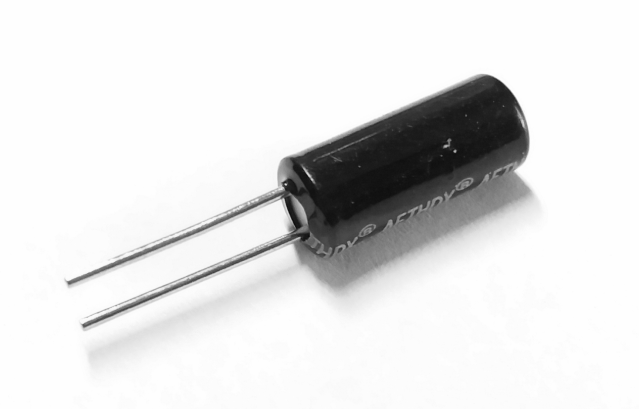
\includegraphics[width=0.2\textwidth]{./pics/neigungsschalter.png}
	\caption{Neigungsschalter.}
	\vspace{-\baselineskip}
\end{wrapfigure}
Mit sogenannten Neigungsschaltern (engl. \emph{tilt switch}) lässt sich eine Neigung, aber auch eine Erschütterung oder der Beginn einer Beschleunigung messen. So lässt sich zum Beispiel feststellen, ob ein Gegenstand angehoben wird.

\begin{ziel}
	\textbf{Ziel:} Es soll eine Alarmanlage gebaut werden, die auslöst, wenn das Steckbrett angehoben wird.
\end{ziel}

\medskip
\begin{aufgabe}
	
	\medskip
	\begin{minipage}{0.59\textwidth}
		Die Abbildung rechts zeigt den Aufbau eines Neigungsschalters im geschlossenen und geöffneten Fall. Beschreibe den Aufbau des Schalters und erkläre, wie es in Abhängigkeit der Neigung des Neigungsschalters zum Leuchten der LED in Abbildung \ref{abb:neigungsschalter-einfach} kommt.
		
		\begin{figure}[H]
			\centering
			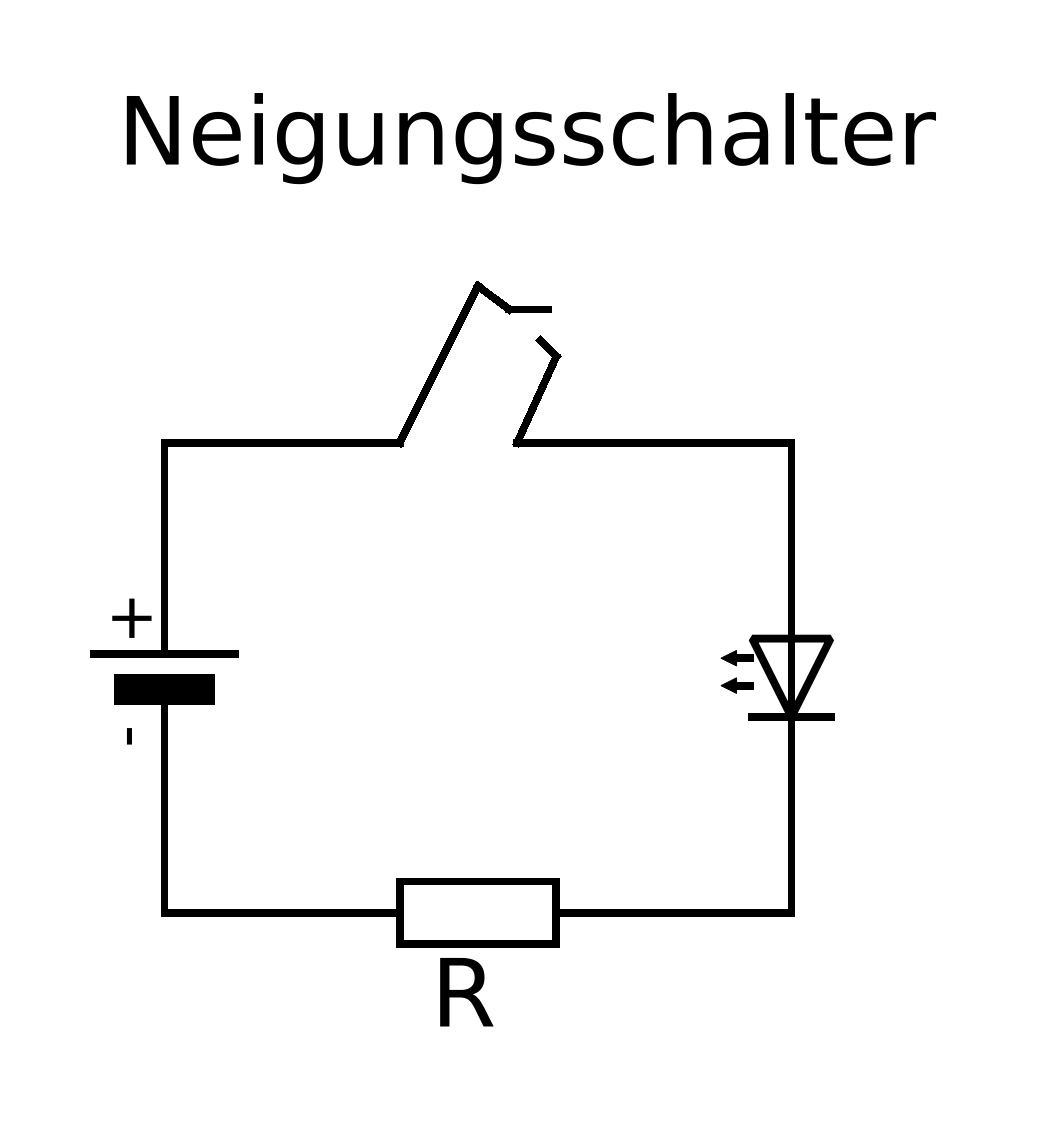
\includegraphics[width=0.4\textwidth]{./Zeichnungen/neigungsschalter-einfach.png}
			\caption{Einfacher Aufbau zum Test eines Neigungsschalters ohne Arduino.}
			\label{abb:neigungsschalter-einfach}
		\end{figure}
	\end{minipage}
	\hfill
	\begin{minipage}{0.39\textwidth}
		\begin{figure}[H]
			\centering
			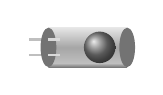
\begin{tikzpicture}
			% Kontaktstifte außen
			\draw [thick, gray!50] (-0.25,0.15) -- (0,0.15);
			\draw [thick, gray!50] (-0.25,0.35) -- (0,0.35);
			% Wände
			\shade [bottom color=gray!95!black, top color=gray!50] (0,0) rectangle (1,0.05);
			\shade [bottom color=gray!50, top color=gray!70] (0,0.05) rectangle (1,0.25);
			\shade [bottom color=gray!70, top color=gray!20] (0,0.25) rectangle (1,0.5);
			% Boden und Deckel
			\fill[gray!90!black] (0,0.25) ellipse [y radius=0.25, x radius=0.1];
			\fill[gray!90!black] (1,0.25) ellipse [y radius=0.25, x radius=0.1];
			% Kontaktstifte innen
			\draw [thick, gray!30] (0,0.15) -- (0.15,0.15);
			\draw [thick, gray!30] (0,0.35) -- (0.15,0.35);
			% Kugel
			\shade [ball color=gray] (0.65,0.25) circle [radius=0.2];
			\end{tikzpicture}
			\caption{Neigungsschalter (geöffnet).}
		\end{figure}
		
		\begin{figure}[H]
			\centering
			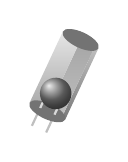
\begin{tikzpicture}[rotate=65]
			% Kontaktstifte außen
			\draw [thick, gray!50] (-0.25,0.15) -- (0,0.15);
			\draw [thick, gray!50] (-0.25,0.35) -- (0,0.35);
			% Wände
			\shade [bottom color=gray!95!black, top color=gray!50] (0,0) rectangle (1,0.05);
			\shade [bottom color=gray!50, top color=gray!70] (0,0.05) rectangle (1,0.25);
			\shade [bottom color=gray!70, top color=gray!20] (0,0.25) rectangle (1,0.5);
			% Boden und Deckel
			\fill[gray!90!black] (0,0.25) ellipse [y radius=0.25, x radius=0.1];
			\fill[gray!90!black] (1,0.25) ellipse [y radius=0.25, x radius=0.1];
			% Kontaktstifte innen
			\draw [thick, gray!30] (0,0.15) -- (0.15,0.15);
			\draw [thick, gray!30] (0,0.35) -- (0.15,0.35);
			% Kugel
			\shade [ball color=gray] (0.25,0.25) circle [radius=0.2];
			\end{tikzpicture}
			\caption{Neigungsschalter (geschlossen).}
		\end{figure}
%		\begin{minipage}[b]{0.49\textwidth}
%			
%		\end{minipage}
%		\hfill
%		\begin{minipage}[b]{0.49\textwidth}
%			
%		\end{minipage}
	\end{minipage}
\end{aufgabe}

\marginpar{%
	\footnotesize%
	\zurueck 
	\hyperref[sec:taster]{Digitale\\ Eingänge}
}
\begin{minipage}[t]{0.55\textwidth}
	\begin{projekt}[Alarmanlage]\label{proj:neigungsalarmanlage}
		Baue eine Alarmanlage, die auslöst, wenn das Steckbrett angehoben wird.
		
		\emph{Hinweis:} Wenn der Neigungsschalter wie rechts abgebildet am Arduino angeschlossen wird, kann sein Zustand in Digitalpin 3 ausgelesen werden (vgl. das \href{sec:taster}{Auslesen von Tastern}).
		
		\emph{Zusatz:} Erkläre, warum es sinnvoll ist, den Piezo-Summer nicht so wie die LED in Abb.\,\ref{abb:neigungsschalter-einfach} direkt mit dem Neigungsschalter zu verbinden, sondern das Auslösen des Tons im Programm zu regeln.
	\end{projekt}
\end{minipage}
\hfill
\begin{minipage}[t]{0.44\textwidth}
	\begin{figure}[H]
		\centering
		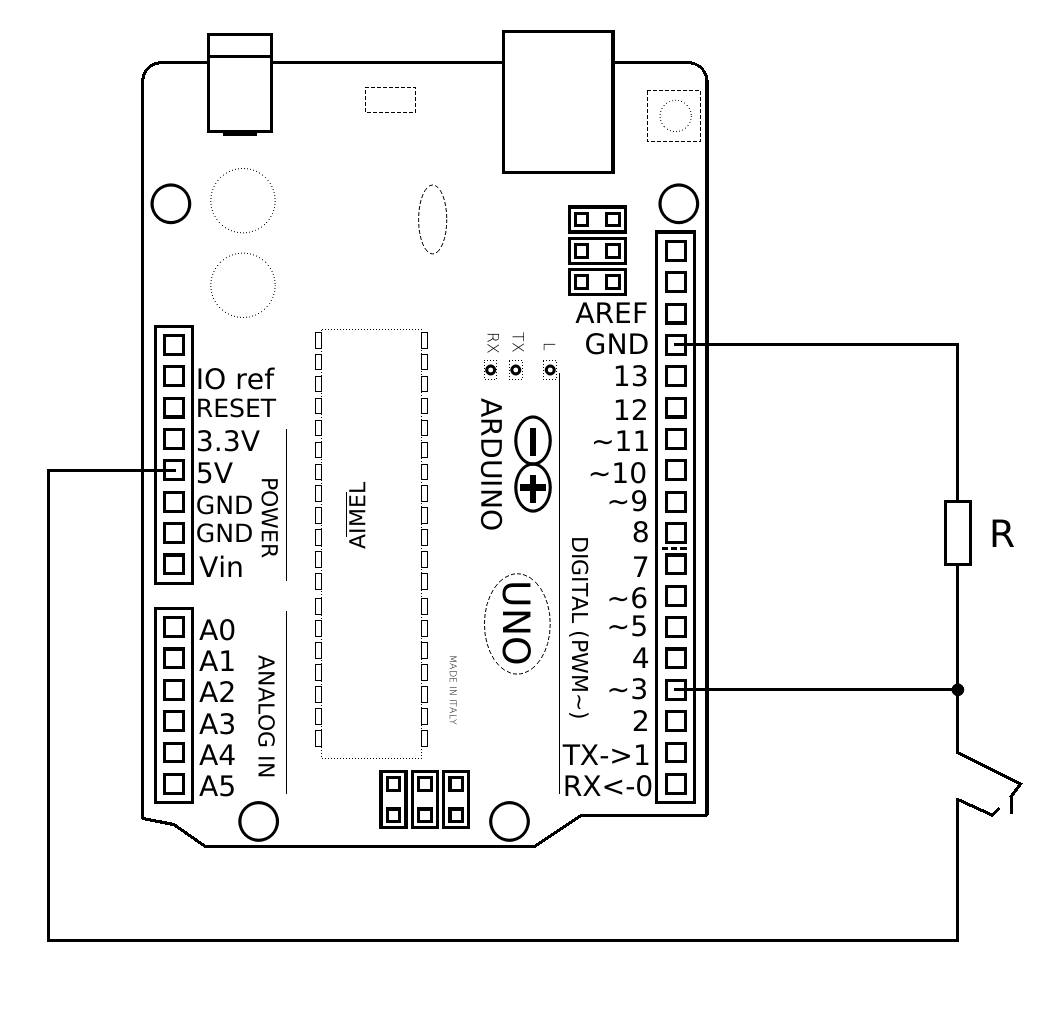
\includegraphics[width=\textwidth]{./Zeichnungen/neigungsschalter-mit-arduino.png}
	\end{figure}
\end{minipage}


\newpage
\section{Bewegungsmelder}
\label{sec:bewegungsmelder}
\setcounter{aufgabennummer}{0}
\setcounter{projektnummer}{0}

\begin{ziel}
	\textbf{Ziel:} Es soll eine Carport-Lampe gebaut werden, die für einige Zeit leuchtet, wenn sie eine Bewegung registriert, und ansonsten dunkel bleibt.
\end{ziel}

\begin{wrapfigure}{r}{0.3\textwidth}
	\centering
	\vspace{-\baselineskip}
	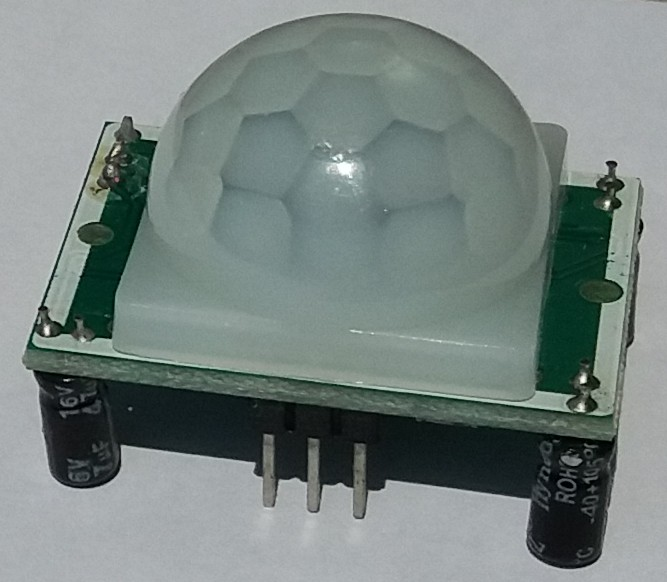
\includegraphics[width=0.2\textwidth]{pics/bewegungsmelder.jpg}
	\label{abb:bewegungsmelder}
	\vspace{-\baselineskip}
\end{wrapfigure}
Bewegungsmelder verfügen über drei Pins, deren Beschriftung man lesen kann, wenn man die Kunststofflinse vorsichtig abzieht (\emph{Vorsicht: Nach Abziehen der Linse nicht den Sensor berühren!}). \texttt{Vcc} und \texttt{GND} dienen der Stromversorgung der elektronischen Komponenten und müssen mit \texttt{5\,V} und \texttt{GND} am Arduino verbunden werden. 

\begin{wrapfigure}{r}{0.3\textwidth}
	\centering
	\vspace{-0.5\baselineskip}
	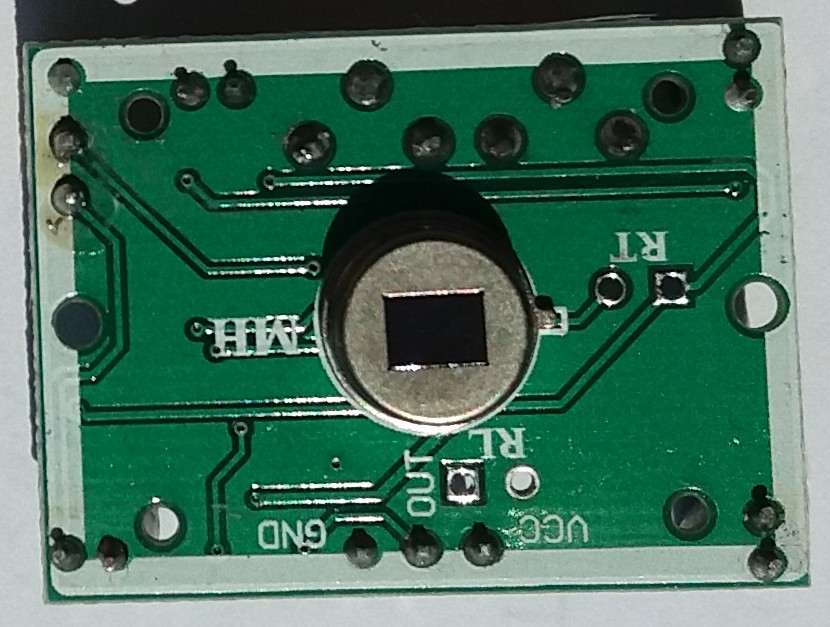
\includegraphics[width=0.25\textwidth]{pics/bewegungsmelder-ohne-linse.jpg}
	\label{abb:bewegungsmelder-ohne-linse}
	\vspace{-0.5\baselineskip}
\end{wrapfigure}
Der mittlere \texttt{OUT}-Pin ist der Signal-Pin: Wenn eine Bewegung registriert wurde, liegt er auf einem hohen elektrischen Potential (\texttt{HIGH}); wenn keine Bewegung registriert wurde, liegt er auf einem niedrigen elektrischen Potential (\texttt{LOW}). Zum Einlesen des Signals wird dieser Pin mit einem digitalen Pin des Arduino verbunden, der dann digitaler Eingang heißt.

\begin{wrapfigure}{r}{0.3\textwidth}
	\centering
	\vspace{-0.75\baselineskip}
	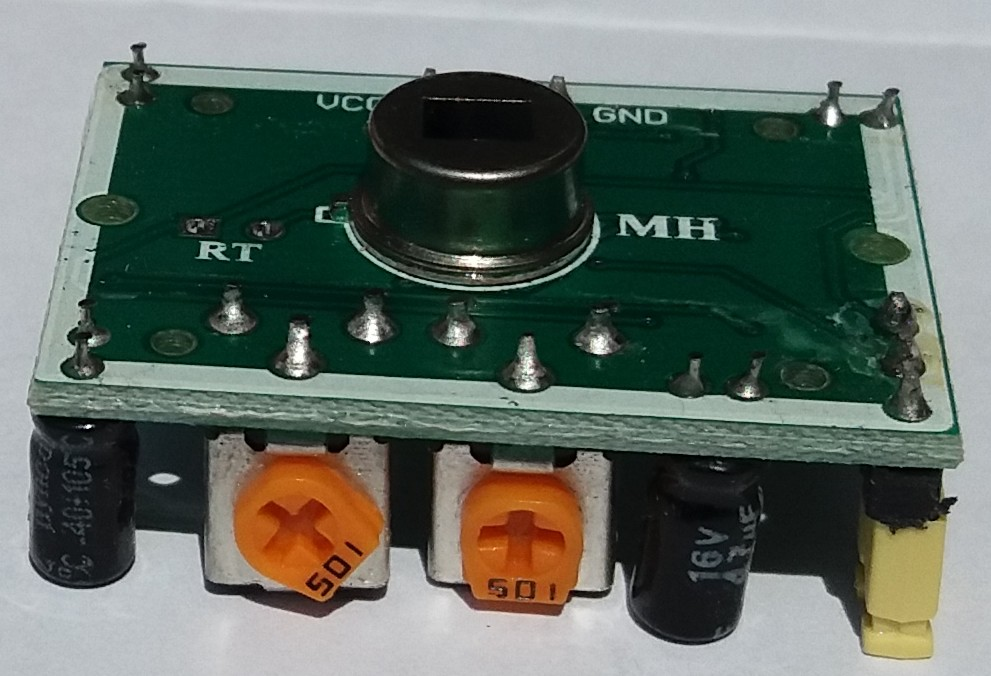
\includegraphics[width=0.25\textwidth]{pics/bewegungsmelder-hinten.jpg}
	\vspace{-\baselineskip}
	\label{abb:bewegungsmelder-hinten}
\end{wrapfigure}
Hinten befinden sich zwei Drehregler (\enquote{Potentiometer}), mit denen sich die Dauer des Bewegungssignals (links) und die Empfindlichkeit (rechts) einstellen lassen. Zusätzlich befindet sich auf der rechten Seite ein sogenannter Jumper, mit dem auf einfache Weise eine Steckverbindung zwischen benachbarten Pins hergestellt werden kann. Wenn sich der Jumper ganz außen befindet, dann bleibt das Bewegungssignal nach dem Erkennen einer Bewegung eine Weile aktiv und wird dann auf jeden Fall deaktiviert. Eine neue Bewegung kann erst nach einer gewissen Zeit wieder registriert werden. Wenn der Jumper hingegen leicht nach innen versetzt ist, bleibt das Bewegungssignal so lange erhalten, wie eine Bewegung erkannt wird (siehe \href{https://funduino.de/nr-8-bewegungsmelder}{Funduino}\footnote{\url{https://funduino.de/nr-8-bewegungsmelder}}).

\begin{projekt}[Carport-Lampe]\label{proj:carport}
	Baue und programmiere eine Carport-Lampe. Experimentiere mit den Drehreglern, um die Empfindlichkeit und Dauer des Signals richtig einzustellen.
\end{projekt}

\marginpar{%
	\footnotesize%
	\zurueck 
	\hyperref[sec:taster]{Digitale\\ Eingänge}
}
\begin{recherche}{Wie funktioniert eigentlich ein Bewegungsmelder?}
	Das zentrale Bauteil eines Bewegungsmelders ist ein sogenannter \emph{Passiver Infrarot Sensor (PIR)}, auch \emph{Pyroelektrischer Sensor}. Recherchiere im Internet, wie solche Sensoren funktionieren und fasse zusammen, wie es zur Registrierung einer Bewegung kommt.	
\end{recherche}

\newpage
\newgeometry{twoside, top=1cm, outer=2.6cm, inner=2.6cm, % inner und outer sind aus irgendeinem Grund vertauscht
	marginparwidth=2cm, marginparsep=0.3cm,% Die Breite für die Marginalien (Randbemerkungen) auf der rechten Seite
	bottom=1cm, footskip=24pt, %Abstand zwischen Textboden und Fußzeilenboden
	includefoot, includehead}
\onehalfspacing
\section{Ultraschallsensor}
\label{sec:ultraschallsensor}
\setcounter{aufgabennummer}{0}
\setcounter{projektnummer}{0}

\marginpar{%
	\footnotesize%
	\zurueck 
	\hyperref[sec:seriellermonitor]{Schleifen \\ Serieller Monitor}
}
Ultraschallsensoren ermöglichen die berührungslose Messung eines Abstands zwischen dem Sensor und dem nächstgelegenen Gegenstand. Dies macht sie zu einer interessanten Ausrüstung für Staubsaugerroboter, die nicht gegen die Wand fahren sollen, oder Einparkhilfen im Auto, die dem Fahrer anzeigen sollen, wie viel Platz er noch hat.

\begin{ziel}
	\textbf{Ziel:} Es soll eine Einparkhilfe für ein Auto gebaut werden.
\end{ziel}

\begin{wrapfigure}{r}{0.35\textwidth}
	\centering
	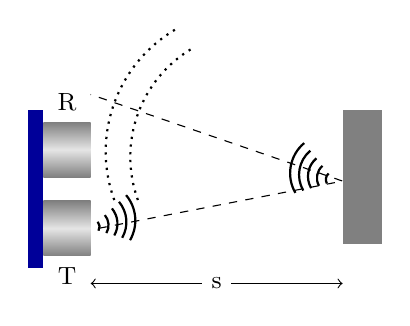
\begin{tikzpicture}
	\fill[blue!60!black] (0,0) rectangle (0.2,2);
	%Transducer
	\shade[bottom color=gray, top color=gray!20!white] (0.2,0.15) rectangle (0.8,0.5);
	\shade[bottom color=gray!20!white, top color=gray] (0.2,0.5) rectangle (0.8,0.85);
	\node at (0.5,-0.1) {\small T};
	% Receiver
	\shade[bottom color=gray, top color=gray!20!white] (0.2,1.15) rectangle (0.8,1.5);
	\shade[bottom color=gray!20!white, top color=gray] (0.2,1.5) rectangle (0.8,1.85);
	\node at (0.5,2.1) {\small R};
	% Schallwelle
	\draw [dashed] (0.9,0.5) -- (4,1.1) -- (0.8,2.2);
	\foreach \x in {1,...,5} {
		\draw [thick] (0.8+\x *0.1,0.5-\x*0.03) arc [start angle=-30, end angle=40, radius=\x mm];
		\draw [thick] (3.9-\x *0.1,1.1-\x*0.03) arc [start angle=210, end angle=130, radius=\x mm];
	}
	\draw [thick,dotted] (3.9-25*0.1,1.1-8*0.03) arc [start angle=200, end angle=120, radius=16 mm];
	\draw [thick,dotted] (3.9-28*0.1,1.1-8*0.03) arc [start angle=200, end angle=120, radius=18 mm];
	%Hindernis
	\fill[gray] (4,0.3) rectangle (4.5,2);
	% Strecke
	\draw [<->] (0.8,-0.2) -- (4,-0.2);
	\node [fill=white] at (2.4,-0.2) {\small s};
	\end{tikzpicture}
\end{wrapfigure}
Die wichtigsten Bestandteile des Ultraschallsensors sind der \enquote{Transducer} (\textbf{T}) und der \enquote{Receiver} (\textbf{R}). Der Transducer ist praktisch ein Lautsprecher, der für uns nicht hörbare Schallwellen aussendet. Der Receiver entspricht einem Mikrofon für Schallwellen. Die Schallwellen werden also vom Transducer ausgesendet, an einem Hindernis reflektiert und vom Receiver empfangen.

Der Ultraschallsensor verfügt über vier Pins. GND und VCC (5\,V) sind wie üblich zu belegen und dienen der Energieversorgung. Der Trigger-Pin dient dazu, einen Ultraschallpuls auszusenden - wird er für 10 Mikrosekunden auf ein HIGH-Potential gebracht, wird der Ultraschallpuls getriggert. Wenn dies geschieht, wird der Echo-Pin von der Elektronik des Sensors auf ein HIGH-Potential gebracht, das so lange anhält, bis der Receiver die reflektierte Schallwelle empfängt. 

Die Zeit, die der Echo-Pin auf HIGH liegt, gibt also an, wie lange der Schall braucht, um vom Sensor zum Hindernis und zurück zu gelangen. Sie kann vom Arduino mithilfe des Befehls 

\button{lese Puls-Pin <\_> Timeout <\_>} gemessen werden. Der Timeout gibt dabei an, nach wie vielen Mikrosekunden der Arduino aufhört, auf eine reflektierte Schallwelle zu warten.

\begin{aufgabe} \emph{Entfernungen messen}
	
	\begin{wrapfigure}{r}{0.48\textwidth}
		\centering
		\vspace{-\baselineskip}
		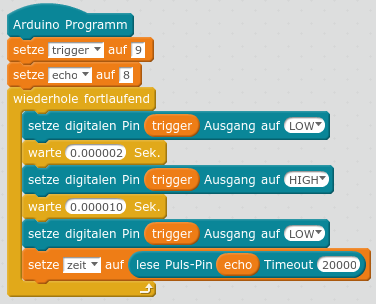
\includegraphics[width=0.48\textwidth]{./pics/ultraschallsensor-start.png}
		\vspace{-\baselineskip}
	\end{wrapfigure}
	Das rechts abgebildete Programm zeigt, wie der Trigger, der mit D9 am Arduino verbunden ist, für genau 10 Mikrosekunden auf HIGH gestellt und dann der Echo-Pin, der mit D8 am Arduino verbunden ist, zur Zeitmessung verwendet wird. In der Variable \texttt{zeit} ist am Ende also die \emph{Zeit in Mikrosekunden} gespeichert, die die Schallwellen vom Sensor zum Hindernis und zurück gebraucht haben.
	
	Erweitere das Programm so, dass die Entfernung vom Mikrocontroller zum Hindernis berechnet und auf dem seriellen Monitor ausgegeben wird. Überprüfe deine Ultraschall-Messung mit dem Geodreieck.
%	\medskip
%	\begin{minipage}{0.48\textwidth}
%		Das rechts abgebildete Programm zeigt, wie der Trigger, der mit D9 am Arduino verbunden ist, für genau 10 Mikrosekunden auf HIGH gestellt und dann der Echo-Pin, der mit D8 am Arduino verbunden ist, zur Zeitmessung verwendet wird. In der Variable \texttt{zeit} ist am Ende also die Zeit in Mikrosekunden gespeichert, die die Schallwellen vom Sensor zum Hindernis und zurück gebraucht haben.
%		
%		Erweitere das Programm so, dass die Entfernung vom Mikrocontroller zum Hindernis berechnet und auf dem seriellen Monitor ausgegeben wird. Überprüfe deine Ultraschall-Messung mit dem Geodreieck.
%	\end{minipage}
%	\hfill
%	\begin{minipage}{0.48\textwidth}
%		\centering
%		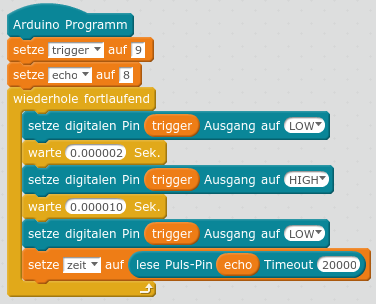
\includegraphics[width=\textwidth]{./pics/ultraschallsensor-start.png}
%	\end{minipage}
	
	\emph{Hinweise:} 
	\begin{itemize}[itemsep=0mm,parsep=0mm]
		\item Schallwellen breiten sich in Luft mit Schallgeschwindigkeit aus - diese beträgt etwa $330\,\frac{\text{m}}{\text{s}}$.
		\item $\SI{1}{\milli\second} = \SI{1000}{\micro\second}$ (Mikrosekunden)
	\end{itemize}
\end{aufgabe}
\restoregeometry
\onehalfspacing

\begin{aufgabe} \emph{Kalibrierung}
	
	Die Schallgeschwindigkeit hängt auch von der Temperatur der Luft ab. Dementsprechend kann es sein, dass die mit dem Wert $330\,\frac{\text{m}}{\text{s}}$ ermittelten Entfernungen (zu) ungenau sind.
	
	Um einen besseren Wert der Schallgeschwindigkeit zu ermitteln, kann man die Strecke zum Hindernis mit einem Geodreieck oder Maßband genau festlegen und die Zeit, die der Schall braucht wie oben beschrieben messen. Bestimme daraus einen besseren Wert für die Schallgeschwindigkeit.
\end{aufgabe}

\begin{projekt}[Einparkhilfe für ein Auto] \label{proj:einparkhilfe}
	Baue eine Einparkhilfe für ein Auto, die umso schneller piepst, je näher man dem Hindernis kommt. Ab einer Entfernung von 30\,cm soll der Ton durchgängig ertönen.
\end{projekt}

\begin{recherche}{Wie wird Ultraschall erzeugt und gemessen?}
	Die Erzeugung des Ultraschalls beruht wie beim Piezo-Summer auf dem inversen piezo-elektrischen Effekt (vgl. S. \pageref{piezo-effekt}); die Messung des Ultraschalls beruht auf dem piezo-elektrischen Effekt. Recherchiere im Internet die Hintergründe dieser Effekte und fasse sie zusammen.
\end{recherche}
\vfill

\newpage
\newgeometry{twoside, top=1cm, outer=2.6cm, inner=2.6cm, % inner und outer sind aus irgendeinem Grund vertauscht
	marginparwidth=2cm, marginparsep=0.3cm,% Die Breite für die Marginalien (Randbemerkungen) auf der rechten Seite
	bottom=1cm, footskip=24pt, %Abstand zwischen Textboden und Fußzeilenboden
	includefoot, includehead}
\onehalfspacing
\section{Liquid Crystal Display (LCD)}
\label{sec:lcd}
\setcounter{aufgabennummer}{0}
\setcounter{projektnummer}{0}
%kurze Übersicht der Befehle
% Hintergrundinfo: Physikalisch - wie werden Pixel sichtbar; informatisch - wie werden Zeichen durch Bitfolgen definiert
% eigene Zeichen definieren: Bsp und Aufgabe
%kein eigenes Projekt: lässt sich bei quasi allen anderen Projekten einbinden

\begin{wrapfigure}{r}{0.3\textwidth}
	\centering
	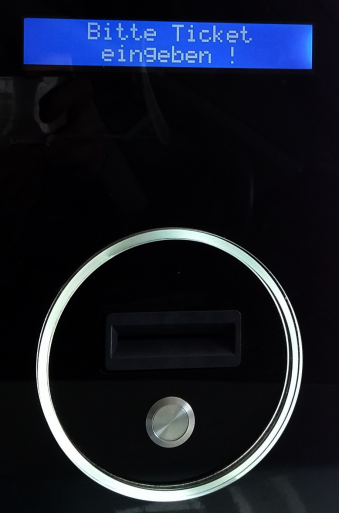
\includegraphics[width=0.3\textwidth]{./pics/lcd-im-parkhaus-v2.png}
	\caption{LC-Display an einem Parkhaus-Automaten.}
	\label{abb:lcd-parkhaus}
	\vspace{-2\baselineskip}
\end{wrapfigure}
In vielen Projekten genügt es nicht, Messwerte, Statusanzeigen oder Menüs über den seriellen Monitor am Computer anzeigen zu lassen - man benötigt stattdessen ein Display, das sich direkt an den Arduino anschließen und mit ihm verbauen lässt. Ein günstige Möglichkeit dafür bieten sogenannte \textbf{L}iquid \textbf{C}rystal \textbf{D}isplays (LCD), die man zum Beispiel in Kaffeemaschinen oder Parkautomaten finden kann (siehe B\ref{abb:lcd-parkhaus}). Modernere LCD werden in Laptops, Fernsehern und Tablets verbaut.

\begin{ziel}
	\textbf{Frage:} Wie verwendet man ein LC-Display am Arduino?
\end{ziel}

Bevor das LC-Display mit mBlock angesteuert werden kann, muss eine Erweiterung installiert werden, die entsprechende Befehle bereitstellt. Die Erweiterung findest du unter \button{Extensions} $\rightarrow$ \button{Extensions verwalten}. Gib im Suchfeld \enquote{lcd} ein und installiere die Erweiterung \enquote{LCD} von Heine Ravnholt.

Die Erweiterung legt fest, an welchen Pins das LC-Display angeschlossen werden muss (siehe unten). Es empfiehlt sich, die zahlreichen 5V- und GND-Anschlüsse auf den Längsseiten des Stecksbretts zu sammeln.

\bigskip
\begin{minipage}{0.64\textwidth}
	\centering
	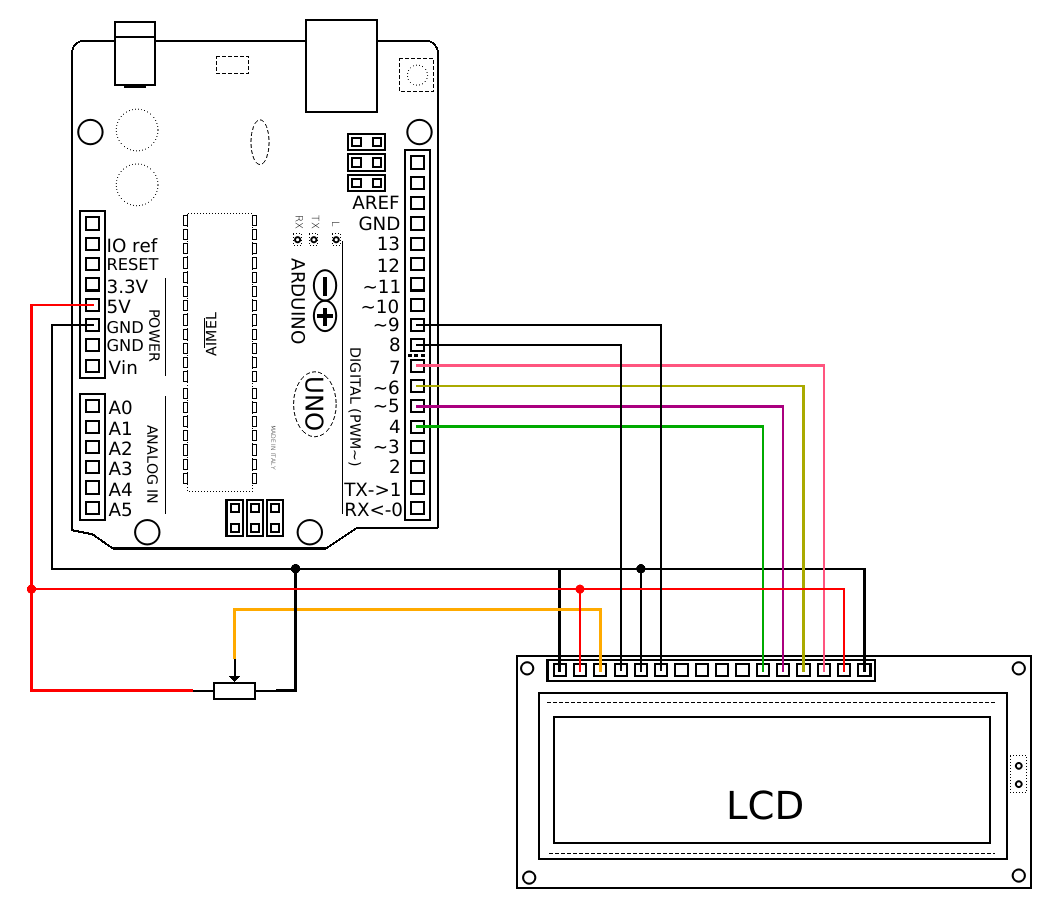
\includegraphics[width=\textwidth]{./Zeichnungen/Schaltplan-Arduino-LCD.png}
\end{minipage}
\hfill
\begin{minipage}{0.34\textwidth}
	\small
	\centering
	\begin{tabular}{c|c}
		\textbf{LCD} & \textbf{Arduino} \\ \hline
		VSS & GND \\ \hline
		VDD & 5V \\ \hline
		V0 & Drehregler (Mitte)\\ \hline
		RS & 8\\ \hline
		RW & GND\\ \hline
		E & 9\\ \hline
		D0 - D3 & -- \\ \hline
		D4 & 4\\ \hline
		D5 & 5\\ \hline
		D6 & 6\\ \hline
		D7 & 7\\ \hline
		A & 5V\\ \hline
		K & GND\\ \hline
	\end{tabular}
\end{minipage}

\bigskip
\begin{aufgabe}\emph{Funktionstest}
			
	Schließe das LC-Display wie beschrieben an den Arduino an und erstelle mithilfe der LCD-Extension ein Programm, das \enquote{Hello World!} auf dem LC-Display anzeigt.
	
	\emph{Hinweis:} Falls alle Pixel weiß oder blau bleiben, kann es sein, dass der Drehregler falsch eingestellt ist. Drehe in diesem Fall an dem Drehregler, um den Kontrast zu verbessern.
\end{aufgabe}
%\begin{minipage}{0.64\textwidth}
%	\begin{aufgabe}\emph{Funktionstest}
%		
%		Schließe das LC-Display wie beschrieben an den Arduino an und erstelle mithilfe der LCD-Extension ein Programm, das \enquote{Hello World!} auf dem LC-Display anzeigt.
%		
%		\emph{Hinweis:} Falls alle Pixel weiß bleiben oder auf dem LCD gar nichts zu sehen ist, kann es sein, dass der Drehregler falsch eingestellt ist. Drehe in diesem Fall an dem Drehregler, um den Kontrast zu verbessern.
%	\end{aufgabe}
%\end{minipage}
%\hfill
%\begin{minipage}{0.34\textwidth}
%	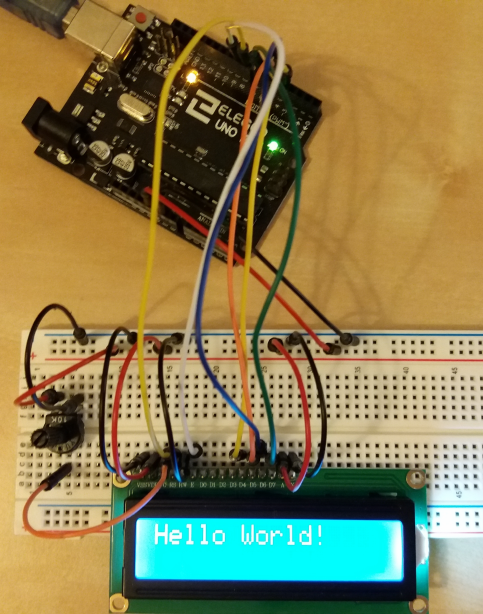
\includegraphics[width=\textwidth]{./pics/arduino-lcd-klein.png}
%\end{minipage}

\newpage
\restoregeometry
\onehalfspacing
% Aufgabe: ständig aktualisierte Anzeige eines Zahlenwertes von 1 bis 300 (rechtsbündig) mit Einheit
\begin{aufgabe} \emph{Messwertanzeige}
	
	In vielen Anwendungen soll auf dem LC-Display ein Messwert o.\,ä. angezeigt werden, der sich mit der Zeit ändern kann. Diese Anzeige soll aber schön formatiert sein.
	
	Erstelle ein Programm, das alle drei Sekunden eine Zufallszahl \texttt{z} zwischen 0 und 200 erzeugt und auf dem Display folgende Anzeige ausgibt:
	
	\begin{center}
		\texttt{Messwert: z E}
	\end{center}
	
	\emph{Hinweise:}
	\begin{itemize}[itemsep=0mm, parsep=0mm]
		\item \texttt{E} soll für eine beliebige Einheit stehen.
		\item Achte darauf, dass der vorherige Wert von \texttt{z} gelöscht wird (\button{lcd clear}).
		\item Die Ausgabe der Zahl \texttt{z} soll immer rechtsbündig erfolgen, sodass zwischen den Einern von \texttt{z} und der Einheit genau ein Leerzeichen steht.
		\item Du benötigst den Befehl \button{LCD set cursor (line <\_> position <\_>)}. Darin steht \texttt{line} für die Zeile, deren Nummer entweder $0$ (oben) oder $1$ (unten) ist. \texttt{position} steht für die Spalte, deren Nummer sich von $0$ bis $15$ erstrecken kann. (In der Informatik beginnt das Zählen stets mit der Null!)		
	\end{itemize}
\end{aufgabe}

\marginpar{%
	\footnotesize%
	\zurueck 
	\hyperref[sec:binaer]{Binär-\\system}
}
\begin{aufgabe} \emph{Codierung von Zeichen auf dem LCD}
	
	In der eingefügten Extension muss im Hintergrund geklärt werden, wie die eingegebenen Zeichen auf dem LCD dargestellt werden. Dazu lohnt ein genauer Blick auf die Zellen des LCD.
	
	Jede Zelle besteht aus $5 \times 8$ Pixeln, von denen manche weiß und manche blau sind. Wenn man für jedes Pixel eine \texttt{1} (weiß) oder eine \texttt{0} (blau) notiert, dann erhält man Bitfolgen (gekennzeichnet durch das vorstehende \texttt{0b}), die sich in einer Reihung notieren lassen.
	
	\begin{figure}[H]
		\centering
		\footnotesize
		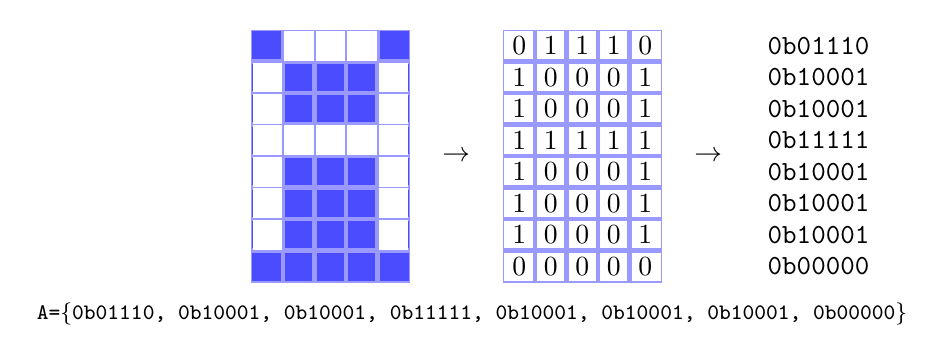
\begin{tikzpicture}[scale=0.4]
		%%%% Zelle auf LCD
		\filldraw[fill=blue!70,draw=blue!40] (0,0) rectangle (5,8);
		\foreach \x in {1,...,4} {
			\draw [blue!40,ultra thick] (\x , 0) -- (\x,8);
		}
		\foreach \y in {1,...,7} {
			\draw [blue!40,ultra thick] (0,\y) -- (5,\y);
		}
		% Zeichen A
		\foreach \x in {0.5,4.5} {
			\foreach \y in {1.5,...,6.5} {
				\fill[white] (\x-0.47,\y-0.47) rectangle (\x+0.47,\y+0.47);
			}
		}
		\foreach \x in {1.5,2.5,3.5} {
			\foreach \y in {4.5,7.5} {
				\fill[white] (\x-0.47,\y-0.47) rectangle (\x+0.47,\y+0.47);
			}
		}
		% Pfeil
		\node at (6.5,4) {$\rightarrow$};
		%%%% Zelle auf LCD codiert
		\filldraw[fill=white,draw=blue!40] (8,0) rectangle (13,8);
		\foreach \x in {9,...,12} {
			\draw [blue!40,ultra thick] (\x , 0) -- (\x,8);
		}
		\foreach \y in {1,...,7} {
			\draw [blue!40,ultra thick] (8,\y) -- (13,\y);
		}
		%Zeichen A codiert
		\foreach \x in {8.5,12.5} {
			\foreach \y in {1.5,...,6.5} {
				\node at (\x,\y) {1};
			}
		}
		\foreach \x in {9.5,10.5,11.5} {
			\foreach \y in {4.5,7.5} {
				\node at (\x,\y) {1};
			}
		}
		\foreach \x in {9.5,10.5,11.5} {
			\foreach \y in {0.5,...,3.5,5.5,6.5} {
				\node at (\x,\y) {0};
			}
		}
		\foreach \x in {8.5,12.5} {
			\foreach \y in {0.5,7.5} {
				\node at (\x,\y) {0};
			}
		}
		% Pfeil
		\node at (14.5,4) {$\rightarrow$};
		%%%% Bitfolgen
		\node at (18,7.5) {\texttt{0b01110}};
		\node at (18,6.5) {\texttt{0b10001}};
		\node at (18,5.5) {\texttt{0b10001}};
		\node at (18,4.5) {\texttt{0b11111}};
		\node at (18,3.5) {\texttt{0b10001}};
		\node at (18,2.5) {\texttt{0b10001}};
		\node at (18,1.5) {\texttt{0b10001}};
		\node at (18,0.5) {\texttt{0b00000}};
		%Zusammenfassung
		\node at (7,-1) {\footnotesize \texttt{A=\{0b01110, 0b10001, 0b10001, 0b11111, 0b10001, 0b10001, 0b10001, 0b00000\}}};
		\end{tikzpicture}
		\caption{Codierung des Buchstabens A auf einem LC-Display.}
	\end{figure}
	
	Man könnte die Reihung von Bitfolgen auch als Reihung von Dezimalzahlen notieren und käme auf das gleiche Ergebnis. Das macht den Code zwar kürzer, jedoch leidet die Lesbarkeit des Codes deutlich.
	
	\emph{Entwerfe einen Smiley und ein eigenes Symbol auf $5 \times 8$ Pixeln und notiere die zugehörige Reihung von Bitfolgen, die dieses Zeichen codiert.}
	
	\emph{Hinweis:} Mit der textbasierten Arduino-IDE lassen sich nach dem oben beschriebenen Prinzip auch eigene Zeichen für das LC-Display codieren. Ein Beispiel findet sich unter \texttt{Datei} $\rightarrow$ \texttt{Beispiele} $\rightarrow$ \texttt{LiquidCrystal} $\rightarrow$ \texttt{CustomCharacter}.
\end{aufgabe}

% Recherche: Physikalischer Hintergrund

\newpage
\section{Servo}
\label{sec:servo}
\setcounter{aufgabennummer}{0}
\setcounter{projektnummer}{0}
\marginpar{%
	\footnotesize%
	\zurueck 
	\hyperref[sec:pwm]{Pulsweitenmodulation}
}
% Tür, die sich öffnet, wenn eine Bewegung registriert wird
\begin{minipage}{0.7\textwidth}
	Ein Servo ist in der Regel ein kleiner Elektromotor zusammen mit einer elektronischen Steuereinheit, die dazu dient, den Motor auf einen bestimmten Winkel einzustellen. Häufig wird beides zusammen als Servomotor bezeichnet. Angewendet werden Servos in vielen Bereichen, zum Beispiel im Modellbau, aber auch in den Fensterhebern von Autos.
\end{minipage}
\hfill
\begin{minipage}{0.28\textwidth}
	\centering
	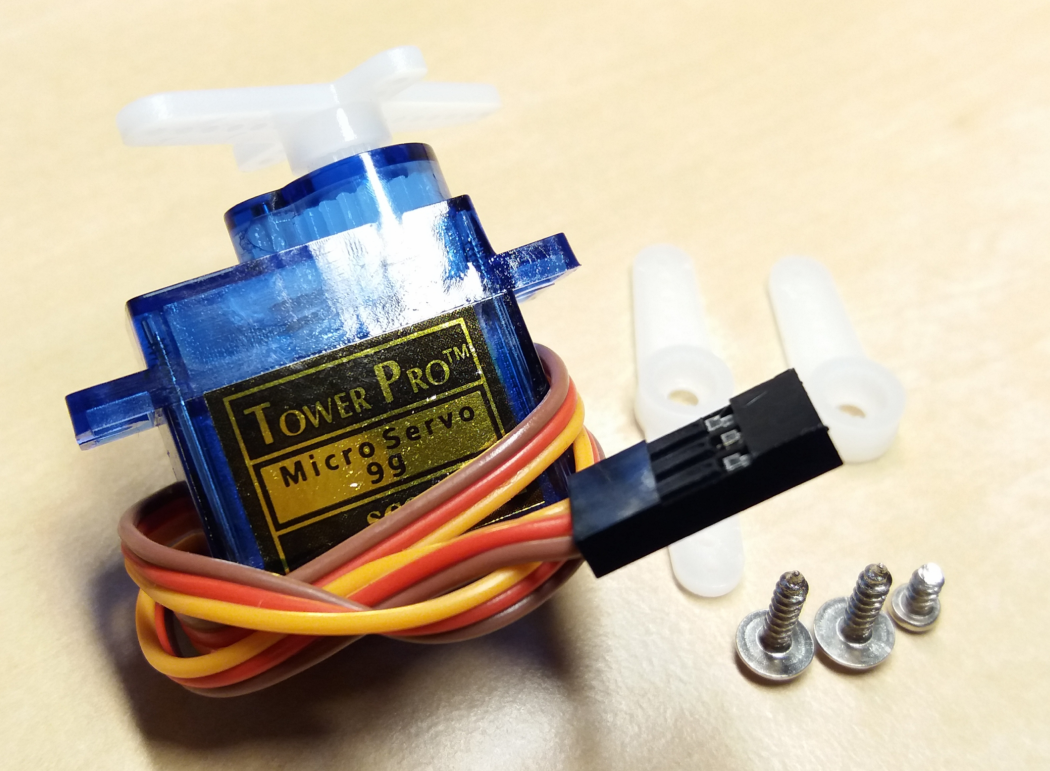
\includegraphics[width=0.9\textwidth]{./pics/servo.png}
\end{minipage}


\begin{figure}[H]
	\centering
	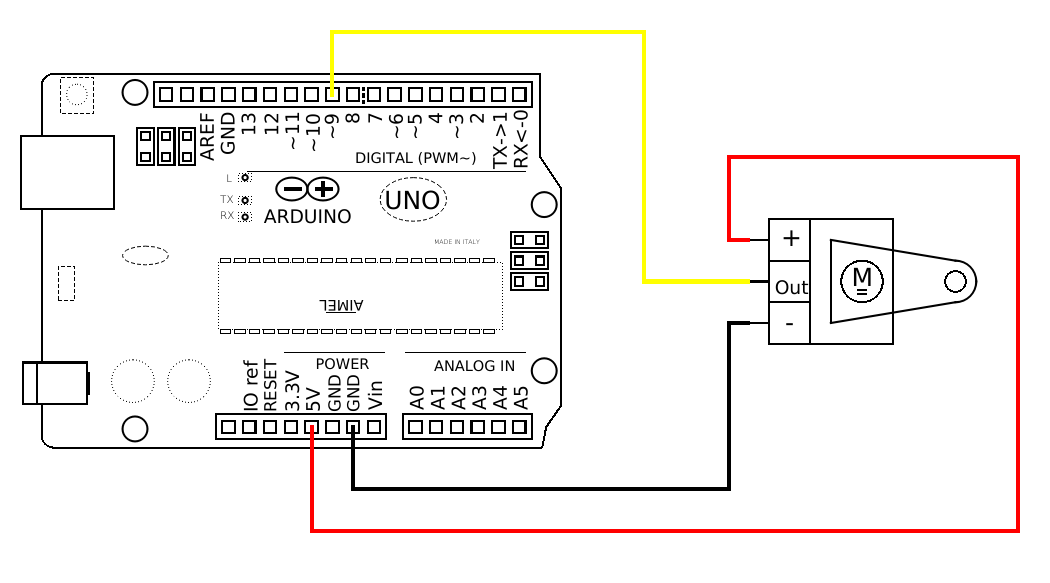
\includegraphics[width=0.7\textwidth]{./Zeichnungen/schaltplan-servo.png}
	\caption{Verschaltung eines Servo am Arduino.}
\end{figure}

Der Servo wird mit drei Anschlüssen an den Arduino angeschlossen:

\begin{itemize}[itemsep=0mm, parsep=0mm]
	\item VCC (rot): Die Stromversorgung des Servo wird mit dem 5\,V-Pin des Arduino verbunden. Dabei ist zu beachten, dass ein Servomotor relativ große Stromstärken \enquote{ziehen} kann. Der 5\,V-Pin des Arduino kann bis zu $\SI{200}{\milli\ampere}$ ausgeben, bevor er durchbrennt. Das ist für den Servo genug. Ein normaler Digitalpin verträgt dagegen nur $\SI{40}{\milli\ampere}$, was deutlich zu wenig für den Servo ist. Die Stromversorgung des Servo kann also nicht über einen normalen Digitalpin sichergestellt werden.
	\item GND (schwarz/braun): Die Stromversorgung ist nur komplett, wenn auch das GND-Niveau auf das GND-Niveau des Arduino festgelegt wird.
	\item Signalleitung (gelb): Die Einstellung des Winkels erfolgt über ein PWM-Signal, deshalb muss das gelbe Kabel mit einem PWM-Pin am Arduino verbunden werden.
\end{itemize}

\begin{projekt}[Uhr]\label{proj:uhr}
	\begin{minipage}{0.6\textwidth}
		Baue mit einem Servo den Sekundenzeiger einer Uhr.		
	\end{minipage}
	\hfill
	\begin{minipage}{0.38\textwidth}
		\centering
		
\includegraphics[width=\textwidth]{./pics/servo-steuerung.png}
	\end{minipage}
\end{projekt}

\begin{projekt}[Fensterheber]\label{proj:fensterheber}
	Der Fensterheber eines Autos hat üblicherweise zwei Funktionen:	
	\begin{enumerate}[label=(\alph*), itemsep=0mm, parsep=0mm]
		\item Wenn man den Schalter halb hochzieht bzw. herunterdrückt, wird das Fenster so lange angehoben bzw. abgesenkt, wie der Schalter in dieser Position verbleibt.
		\item Wenn der Schalter ganz hochgezogen bzw. heruntergedrückt wird, wird das Fenster auch ganz hochgehoben bzw. heruntergefahren.
	\end{enumerate}

	Modelliere eine Funktion des Fensterhebers mit zwei Tastern (mit Widerstand! - vgl. Abschnitt \ref{sec:taster}) und einem Servo. Wenn du beide Funktionen modellieren willst, brauchst du vier Taster (mit Widerstand!).
\end{projekt}

\begin{recherche}{Wie funktioniert die Steuerung eines Servos?}
	Der Winkel, auf den sich die Ausgangswelle des Servo drehen soll, wird über ein PWM-Signal geregelt. Recherchiere im Internet, wie dies realisiert wird und fasse es zusammen.
\end{recherche}

\newpage
\section{Joystick}
\label{sec:joystick}
\setcounter{aufgabennummer}{0}
\setcounter{projektnummer}{0}
\marginpar{%
	\footnotesize%
	\zurueck 
	\hyperref[sec:potentiometer]{Potentiometer}
}
Joysticks werden bekanntermaßen für Spielecontroller oder auch zur Steuerung von Maschinen genutzt. Mit dem Arduino lassen sich einfache Versionen davon nachbauen.

\begin{ziel}
	\textbf{Frage:} Wie funktioniert ein Joystick und wie verwendet man ein Joystick-Modul am Arduino?
\end{ziel}

\medskip
\begin{minipage}{0.73\textwidth}
	Ein Joystick besteht im Wesentlichen aus zwei Potentiometern, die über einen gemeinsamen Hebel variiert werden können. Wie im Schaltbild zu sehen, teilen sich beide den 5V- und GND-Anschluss; der mittlere Anschluss muss natürlich jeweils einzeln ausgelesen werden. Zusätzlich wird durch Drücken des Joysticks ein angebrachter Taster gedrückt, dessen Status am SW-Pin ausgelesen werden kann (\emph{sw von engl. \enquote{switch}}). Da das elektrische Potential am SW-Pin normalerweise schwankt, sollte ein \emph{Pullup}-Widerstand mit $R=\SI{1}{\kilo\ohm}$ angebracht werden (vgl. Schaltbild).	
\end{minipage}
\hfill
\begin{minipage}{0.25\textwidth}
	\centering
	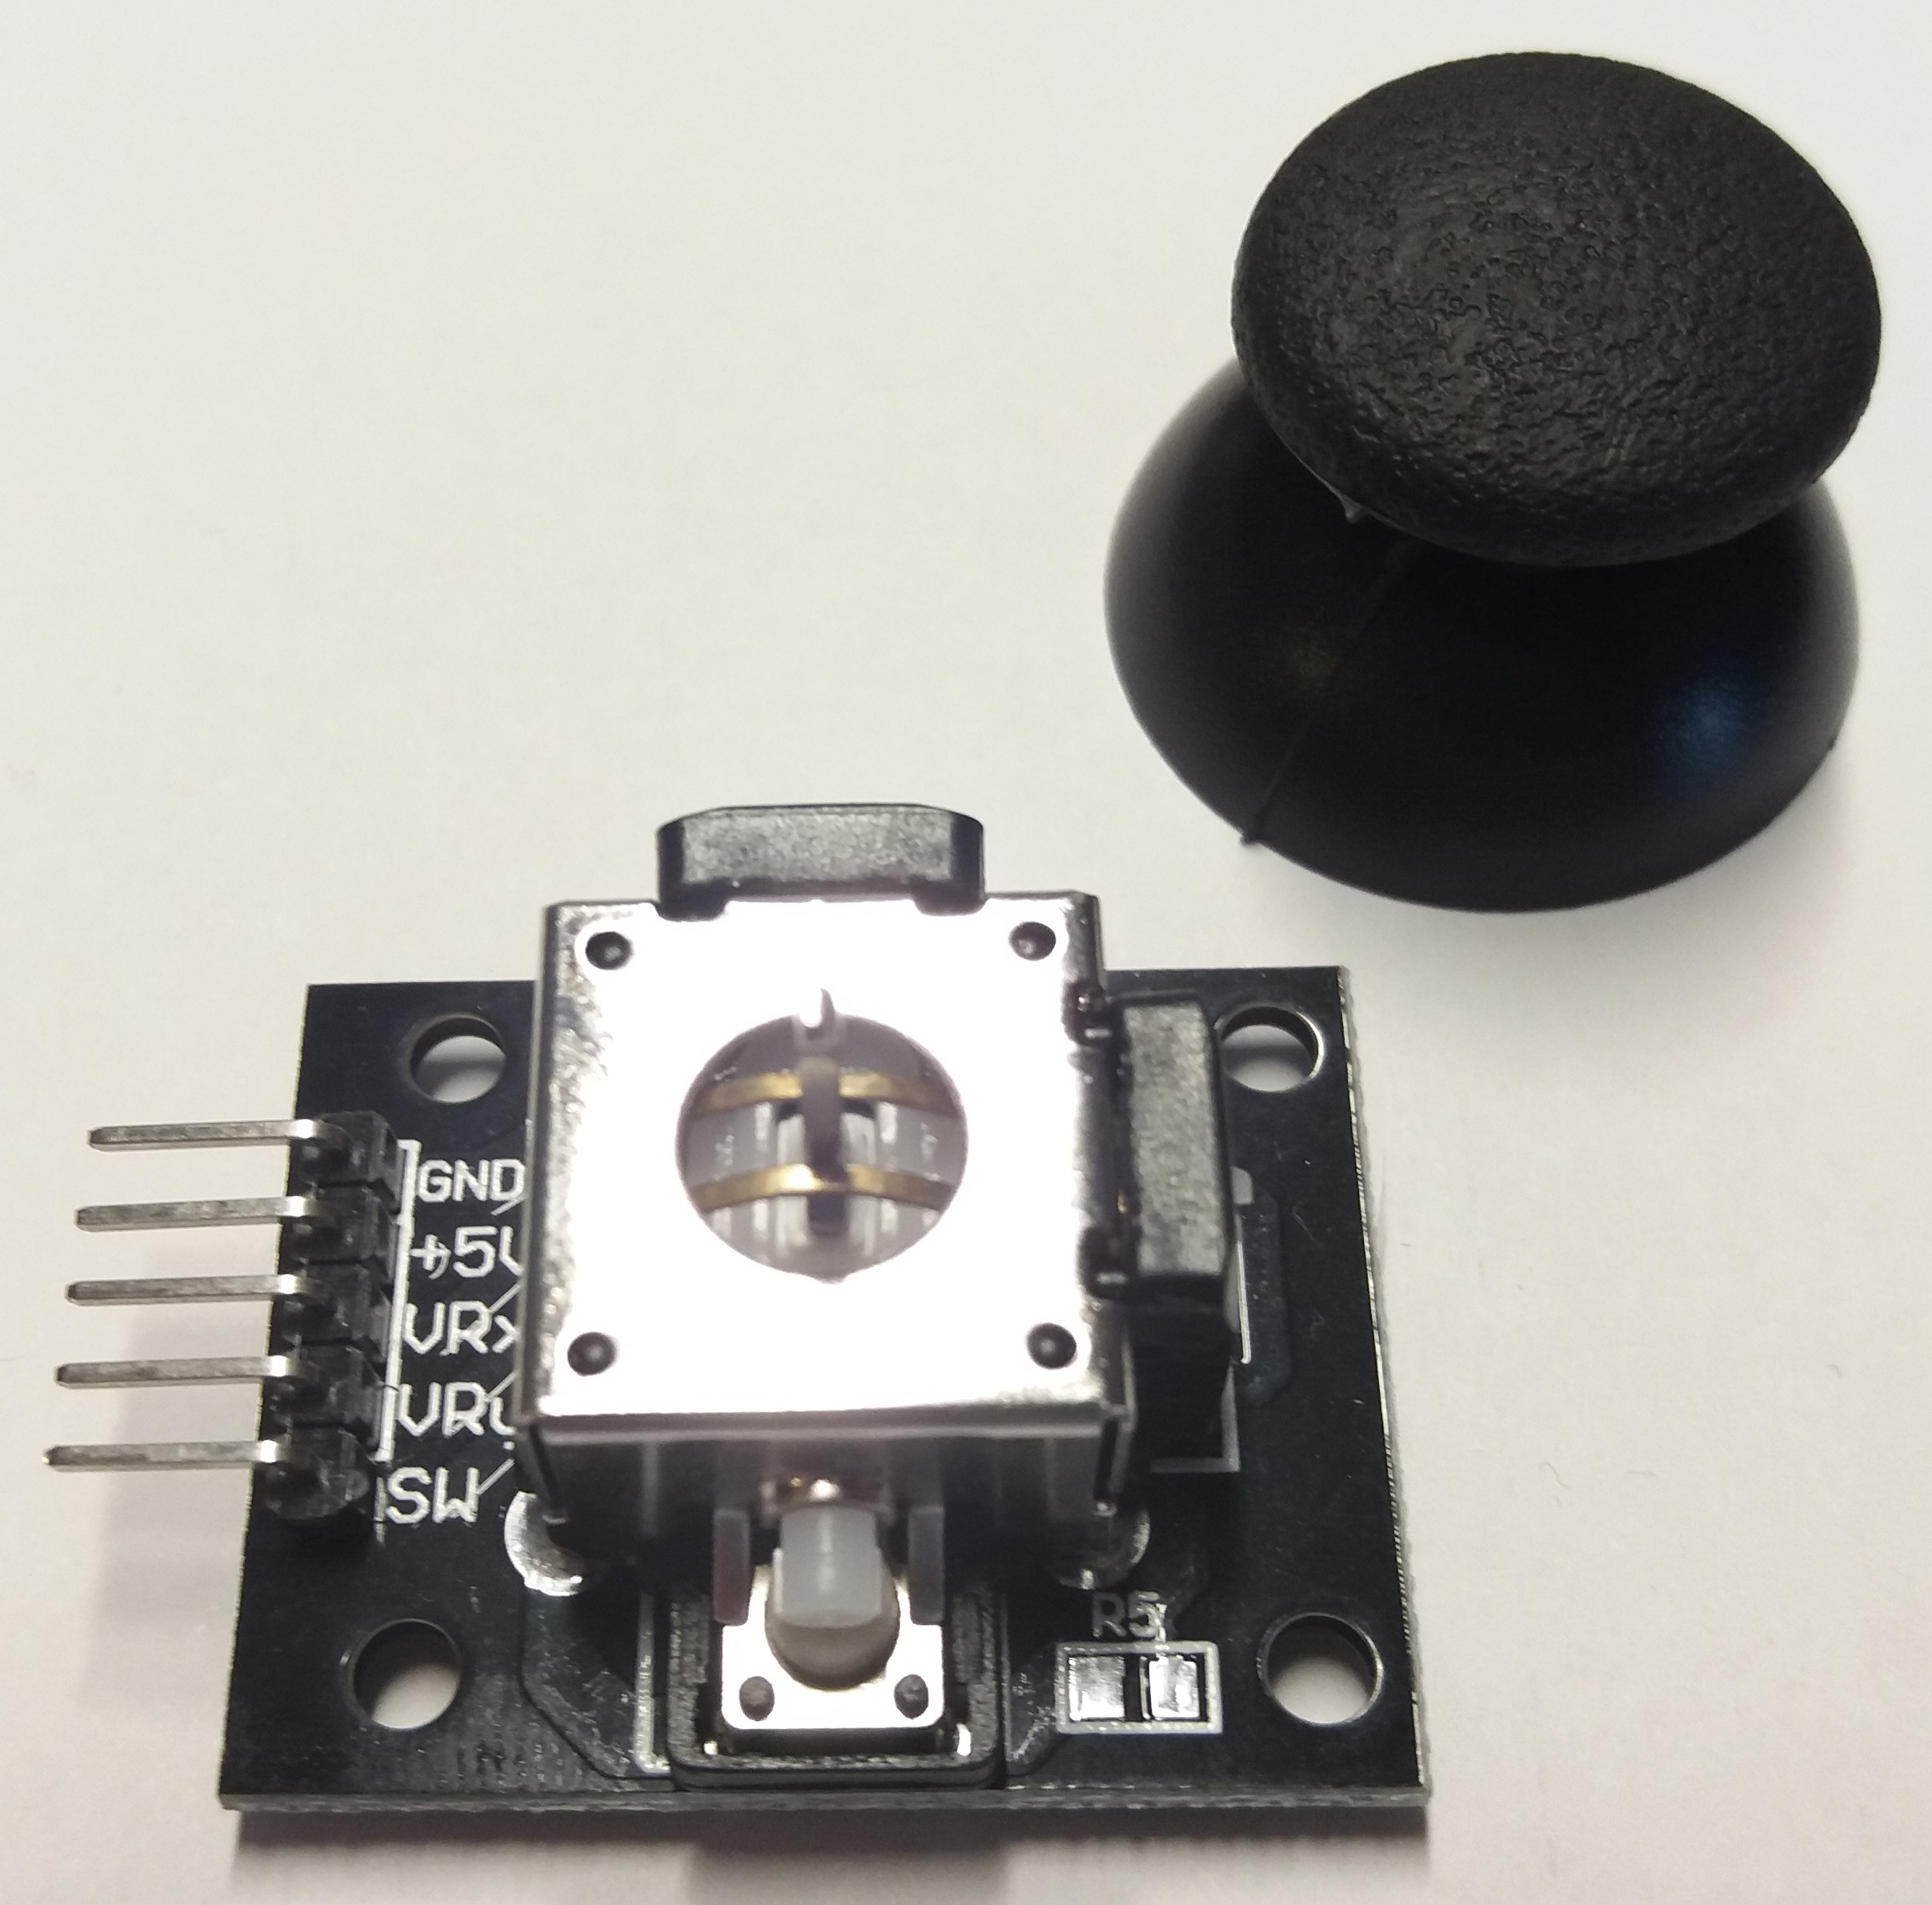
\includegraphics[width=\linewidth]{./pics/joystick.jpg}
\end{minipage}

\begin{figure}[H]
	\hfill
	\begin{minipage}{0.48\textwidth}
		\centering
		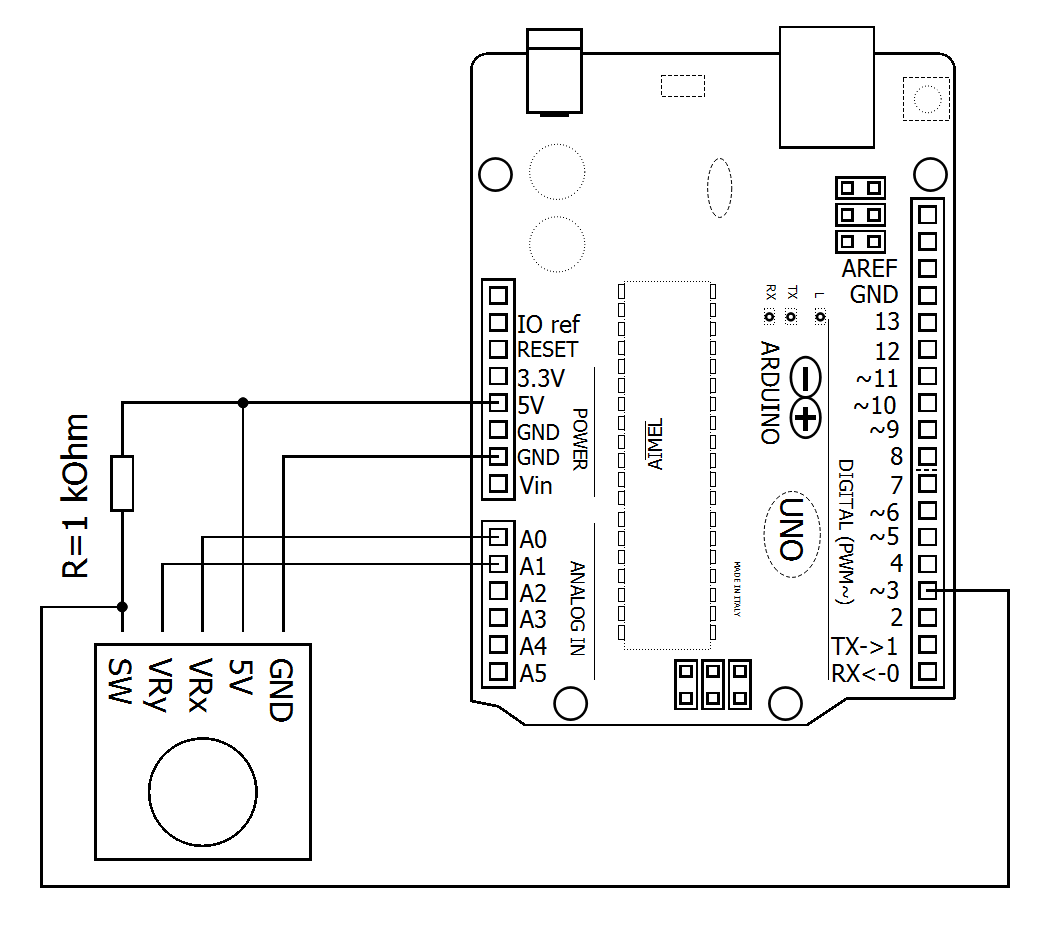
\includegraphics[width=\textwidth]{./Zeichnungen/Schaltplan-Joystick.png}
		\caption{Anschluss des Joystick-Moduls an den Arduino.}
	\end{minipage}
	\hfill
	\begin{minipage}{0.38\textwidth}
		\centering
		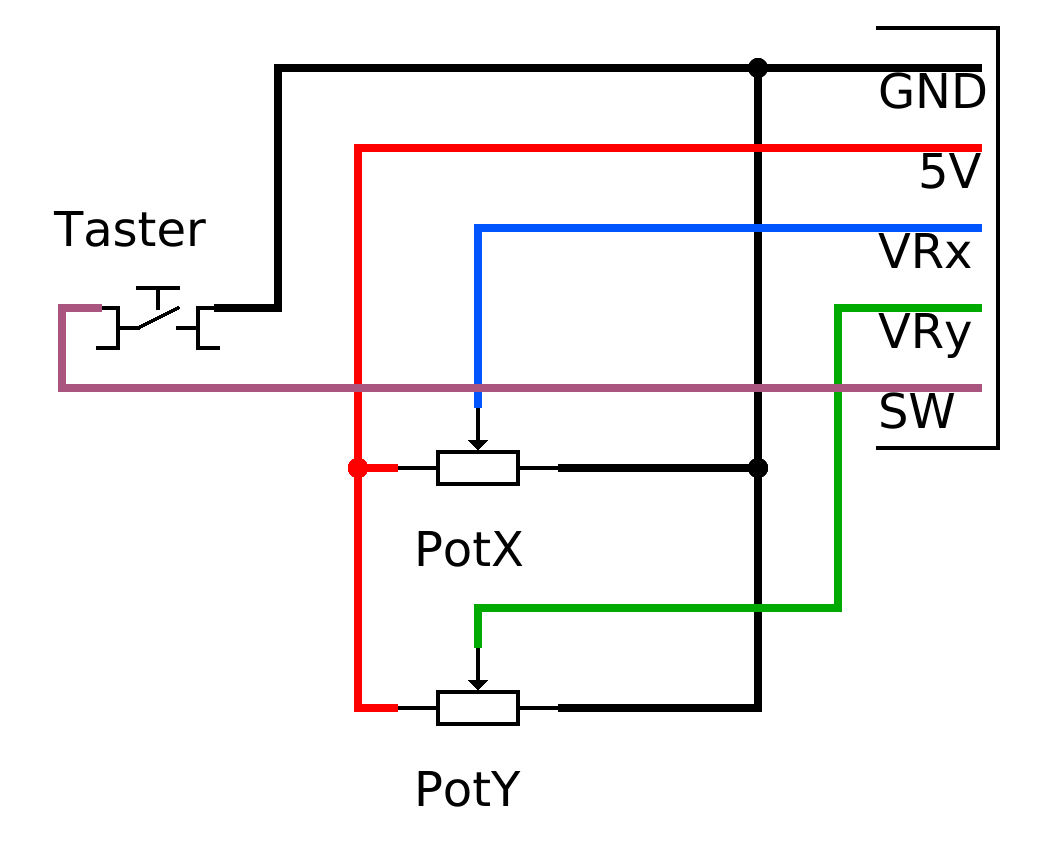
\includegraphics[width=\textwidth]{./Zeichnungen/Schaltplan-Joystick-Ersatz.png}
		\caption{Ersatzschaltplan für das Joystick-Modul.}
	\end{minipage}
	\hfill
\end{figure}

\begin{aufgabe} \emph{Erste Experimente}
	\begin{enumerate}[label=\alph*), itemsep=0ex,parsep=0ex]
		\item Bewege den Hebel des Joystick-Moduls und beobachte, wie sich dabei die Potentiometer an den Seiten mitbewegen. Bringe auch den Plastikdeckel an, drücke den Joystick herunter und beobachte dabei das Verhalten des Tasters.
		\item Schließe das Joystick-Modul wie oben beschrieben an den Arduino an. Lies die Werte der Potentiometer aus, während du sie bewegst. Notiere, welche Bewegungsrichtung die X-Richtung und welche die Y-Richtung darstellt. Notiere außerdem, welches der beiden Potentiometer (ggü. von Taster oder ggü. der Pins) für die X-Richtung bzw. Y-Richtung verantwortlich ist.
		\item Mit dem Pullup-Widerstand wird eine sogenannte Active-Low Schaltung aufgebaut. Teste die Funktionsweise des Tasters, indem du das elektrische Potential in D3 ausliest und beschreibe, was mit dem Begriff Active-Low gemeint ist.
	\end{enumerate}
\end{aufgabe}
% El Potential an SW (Taster) schwankt ohne Pullup stark; mit Pullup wird es im offenen Fall auf 5V gezogen, im geschlossenen Fall auf 0V.
% Active-LOW: Durch Drücken wird ein 0V-Potential gelesen, also 0 oder FALSE. Das Verhalten ist genau anders herum wie man es erwarten würde.
% x-Koordinate: Veränderung durch Verschiebung in Richtung der Kabel bzw. davon weg (Poti gegenüber von Taster) (auslesen an analogem Eingang)
% y-Koordinate: Veränderung durch Verschiebung in Richtung des Tasters bzw. davon weg (Poti gegenüber der Kabel) (auslesen an analogem Eingang)

\begin{projekt}[Joystick-RGB-Steuerung]\label{proj:joystick-rgb}
	Steuere mit dem Joystick-Modul die Farbe einer RGB-LED!
	
	\emph{\footnotesize Da man nur zwei Freiheitsgrade bzw. Bewegungsrichtungen hat, lassen sich leider nicht alle Farbanteile mit dem Joystick-Modul kontrollieren. Interessant sieht das Ergebnis trotzdem aus.}
\end{projekt}


\textbf{Achtung bei Verwendung von Motoren:}\marginpar{\centering\ausrufezeichen} Es wäre natürlich reizvoll, mit dem Joystick-Modul und zwei Servos oder Motoren einen Roboter-Arm zu steuern. Der Arduino allein kann aber weder zwei Servos noch zwei einfache Elektromotoren mit Strom versorgen. Wie eine solche Schaltung zu realisieren wäre, zeigt Kapitel \ref{kap:elektromotoren}.

\newpage
\section{Infrarot-Fernbedienung}
\label{sec:infrarot-fern}
\setcounter{aufgabennummer}{0}
\setcounter{projektnummer}{0}
\marginpar{%
	\footnotesize%
	\zurueck 
	\hyperref[sec:ldr]{Helligkeit messen}
}
Jeder weiß, wie angenehm es ist, wenn man ein Gerät fernsteuern kann statt aufstehen zu müssen, um die angebrachten Knöpfe zu drücken. Eine einfache Möglichkeit dafür bietet eine Infrarot(IR)-Fernbedienung.

\begin{ziel}
	\textbf{Frage:} Wie verwendet man eine IR-Fernbedienung mit dem Arduino?
\end{ziel}

Wie am Namen zu erkennen, verwendet eine IR-Fernbedienung Infrarotstrahlen, die mit dem bloßen Auge nicht sichtbar sind. Hält man jedoch eine Digitalkamera, z.\,B. vom Smartphone, auf die Infrarot-LED der Fernbedienung und drückt eine Taste, dann kann man ein schnelles Aufblitzen erkennen. Am besten probierst du es selbst einmal aus oder schaust dir ein kurzes \video \href{https://el-voss.de/downloads/ir-strahlen.html}{Video der IR-Strahlen} an. Das Aufblitzen zeigt, dass die Strahlen in einem bestimmten Rhythmus gesendet werden, aus dem sich entschlüsseln lässt, welche Taste gedrückt wurde.

\medskip
\begin{minipage}{0.7\textwidth}
	Empfangen werden die Infrarotstrahlen von einem IR-Empfängermodul, das unter anderem eine Fotozelle enthält, die im Gegensatz zum LDR nicht auf das sichtbare Licht reagiert, sondern auf Infrarotlicht bei einer Frequenz von $\SI{38}{\kilo\hertz}$. Der Anschluss an den Arduino ist einfach: GND und 5V dienen wie üblich der Stromversorgung. Der Signal-Pin S muss mit einem beliebigen PWM-Pin (mit $\sim$) verbunden werden.
\end{minipage}
\hfill
\begin{minipage}{0.28\textwidth}
	\begin{figure}[H]
		\centering
		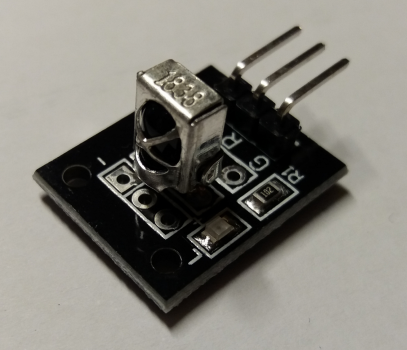
\includegraphics[width=0.7\textwidth]{./pics/ir-led.png}
		\caption{IR-Empfängermodul.}
	\end{figure}	
\end{minipage}
\medskip

\begin{figure}[H]
	\centering
	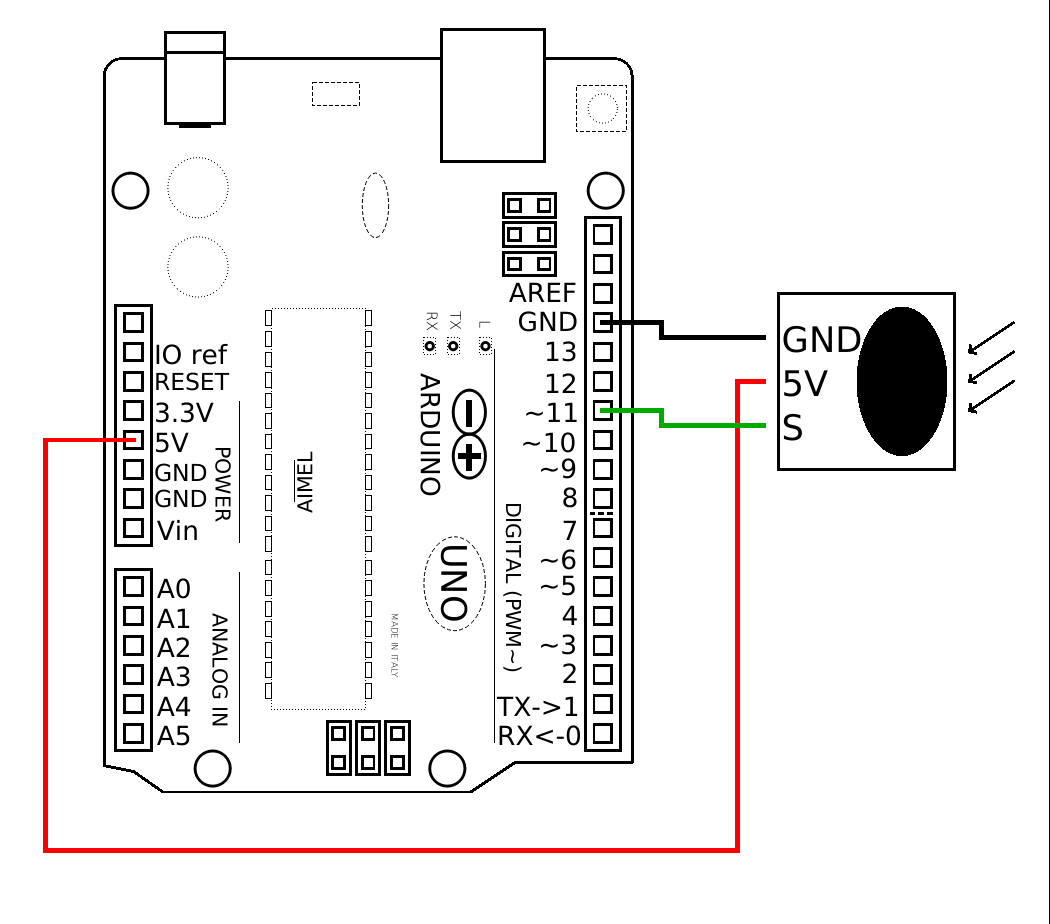
\includegraphics[width=0.4\textwidth]{./Zeichnungen/Schaltplan-IR-Empfaenger.png}
	\caption{Schaltplan zum Anschluss des IR-Empfängermoduls am Arduino.}
\end{figure}

Zum Einlesen und Entschlüsseln des Signals sollte die Erweiterung \enquote{IR Remote} von AbbadoN installiert werden. Dazu wählt man \button{Extensions} $\rightarrow$ \button{Extensions verwalten} und sucht nach \enquote{ir remote}.

Mithilfe der Befehle aus der Erweiterung lässt sich das Drücken der Fernbedienung wie unten abgebildet auslesen:
\begin{itemize}[itemsep=0mm,parsep=0mm]
	\item Mit \button{IRremote pin(<\_>)} wird ein IR-Empfänger initialisiert, dessen Signalpin im rechts abgebildeten Beispiel mit Pin 11 verbunden ist.
	\item Der Befehl \button{bulean result receive} (Achtung: \enquote{boolean} wurde dort falsch geschrieben) gibt \texttt{TRUE} zurück, wenn ein neues Signal empfangen wurde, ansonsten \texttt{FALSE}.
	\item Das decodierte Signal ist eine Zahl, auf deren Wert man mit \button{Value Results} zugreifen kann. Dies kann zum Beispiel auf dem seriellen Monitor angezeigt werden. Alternativ oder zusätzlich kann durch eine Abfrage des Codes die LED an Pin 13 an bzw. ausgeschaltet werden (im Beispiel rechts mit den Tasten 1 und 2).
	\item Mit \button{Resume IR receive} wird der Wert von \texttt{Value Results} wieder zurückgesetzt und das IR-Empfängermodul wieder in den Empfangsmodus versetzt. Dieser Befehl sollte daher immer als Letztes nach der Verarbeitung des Signals erfolgen.
\end{itemize}

\begin{figure}[H]
	\centering
	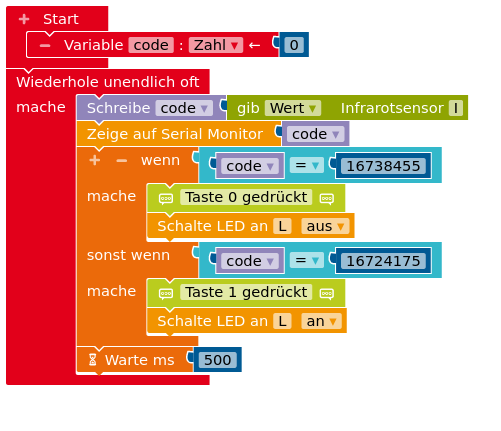
\includegraphics[width=0.5\textwidth]{./pics/ir-fernbedienung-auslesen.png}
	\caption{Einfaches Beispielprogramm zur Verwendung einer IR-Fernbedienung.}
\end{figure}

%\par
%\begin{minipage}{0.58\textwidth}
%	Mithilfe der Befehle aus der Erweiterung lässt sich das Drücken der Fernbedienung wie rechts abgebildet auslesen:
%	\begin{itemize}[itemsep=0mm,parsep=0mm]
%		\item Mit \button{IRremote pin(<\_>)} wird ein IR-Empfänger initialisiert, dessen Signalpin im rechts abgebildeten Beispiel mit Pin 11 verbunden ist.
%		\item Der Befehl \button{bulean result receive} (Achtung: \enquote{boolean} wurde dort falsch geschrieben) gibt \texttt{TRUE} zurück, wenn ein neues Signal empfangen wurde, ansonsten \texttt{FALSE}.
%		\item Das decodierte Signal ist eine Zahl, auf deren Wert man mit \button{Value Results} zugreifen kann. Dies kann zum Beispiel auf dem seriellen Monitor angezeigt werden. Alternativ oder zusätzlich kann durch eine Abfrage des Codes die LED an Pin 13 an bzw. ausgeschaltet werden (im Beispiel rechts mit den Tasten 1 und 2).
%		\item Mit \button{Resume IR receive} wird der Wert von \texttt{Value Results} wieder zurückgesetzt und das IR-Empfängermodul wieder in den Empfangsmodus versetzt. Dieser Befehl sollte daher immer als Letztes nach der Verarbeitung des Signals erfolgen.
%	\end{itemize}
%\end{minipage}
%\hfill
%\begin{minipage}{0.4\textwidth}
%	\begin{figure}[H]
%		\centering
%		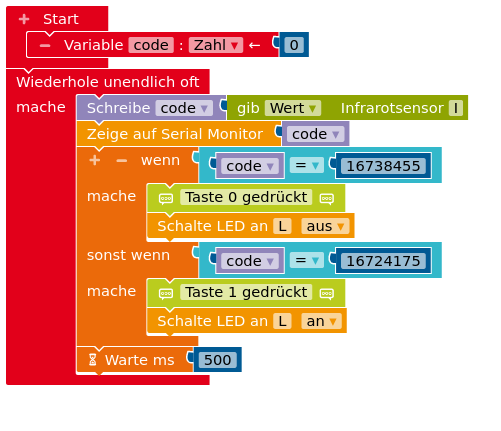
\includegraphics[width=\textwidth]{./pics/ir-fernbedienung-auslesen.png}
%	\end{figure}	
%\end{minipage}
%\par

\begin{aufgabe} \emph{Codes kennen lernen}
	\begin{enumerate}[label=\alph*),itemsep=0mm,parsep=0mm]
		\item Übertrage das oben abgebildete Programm auf den Arduino und probiere es aus.
		\item Erstelle eine Tabelle, in der du den Zahlencode für jede Taste festhälst. Probiere auch aus, was passiert, wenn du die Tasten länger gedrückt hälst.
	\end{enumerate}
\end{aufgabe}

\marginpar{%
	\footnotesize%
	\video \\
	\href{https://www.youtube.com/watch?v=1PUyE8QJuAw}{Lichterkette-Beispielvideo}
}
\begin{projekt}[Fernsteuerung eines RGB-LED-Streifens]\label{proj:fernsteuerung-rgb}
	In vielen Bereichen werden RGB-LED-Streifen genutzt, um einen Raum mit passendem, indirektem Licht auszustatten. Die meisten RGB-Streifen lassen sich über eine kleine Infrarot-Fernbedienung steuern, wodurch sich die Farbe, aber auch der Modus einstellen lässt - zum Beispiel eine einzelne Farbe, \hyperref[sec:pwm]{Fading}, Strobe, \dots
	
	Die einzelnen LEDs machen dabei alle dasselbe. Es reicht also für einen Prototypen, das Muster mit einer RGB-LED nachzubauen. Programmiere die verschiedenen Modi so, dass sie sich über die Fernbedienung steuern lassen.
\end{projekt}

\newpage
\section{Temperatur- und Luftfeuchtigkeitssensor DHT-11}
\label{sec:templuft}
\setcounter{aufgabennummer}{0}
\setcounter{projektnummer}{0}

\marginpar{%
	\footnotesize%
	\zurueck 
	\hyperref[sec:ntc]{Temperatur messen}
}
\begin{minipage}{0.7\textwidth}
	Bei vielen Umweltmessungen interessiert nicht nur die Temperatur, sondern auch die Luftfeuchtigkeit. Der Sensor DHT-11 ist ein einfaches, kleines Bauteil, mit dem sich beides messen lässt.
	
	\begin{ziel}
		\textbf{Frage:} Wie verwendet man den DHT-11 am Arduino?
	\end{ziel}
\end{minipage}
\hfill
\begin{minipage}{0.25\textwidth}
	\centering
	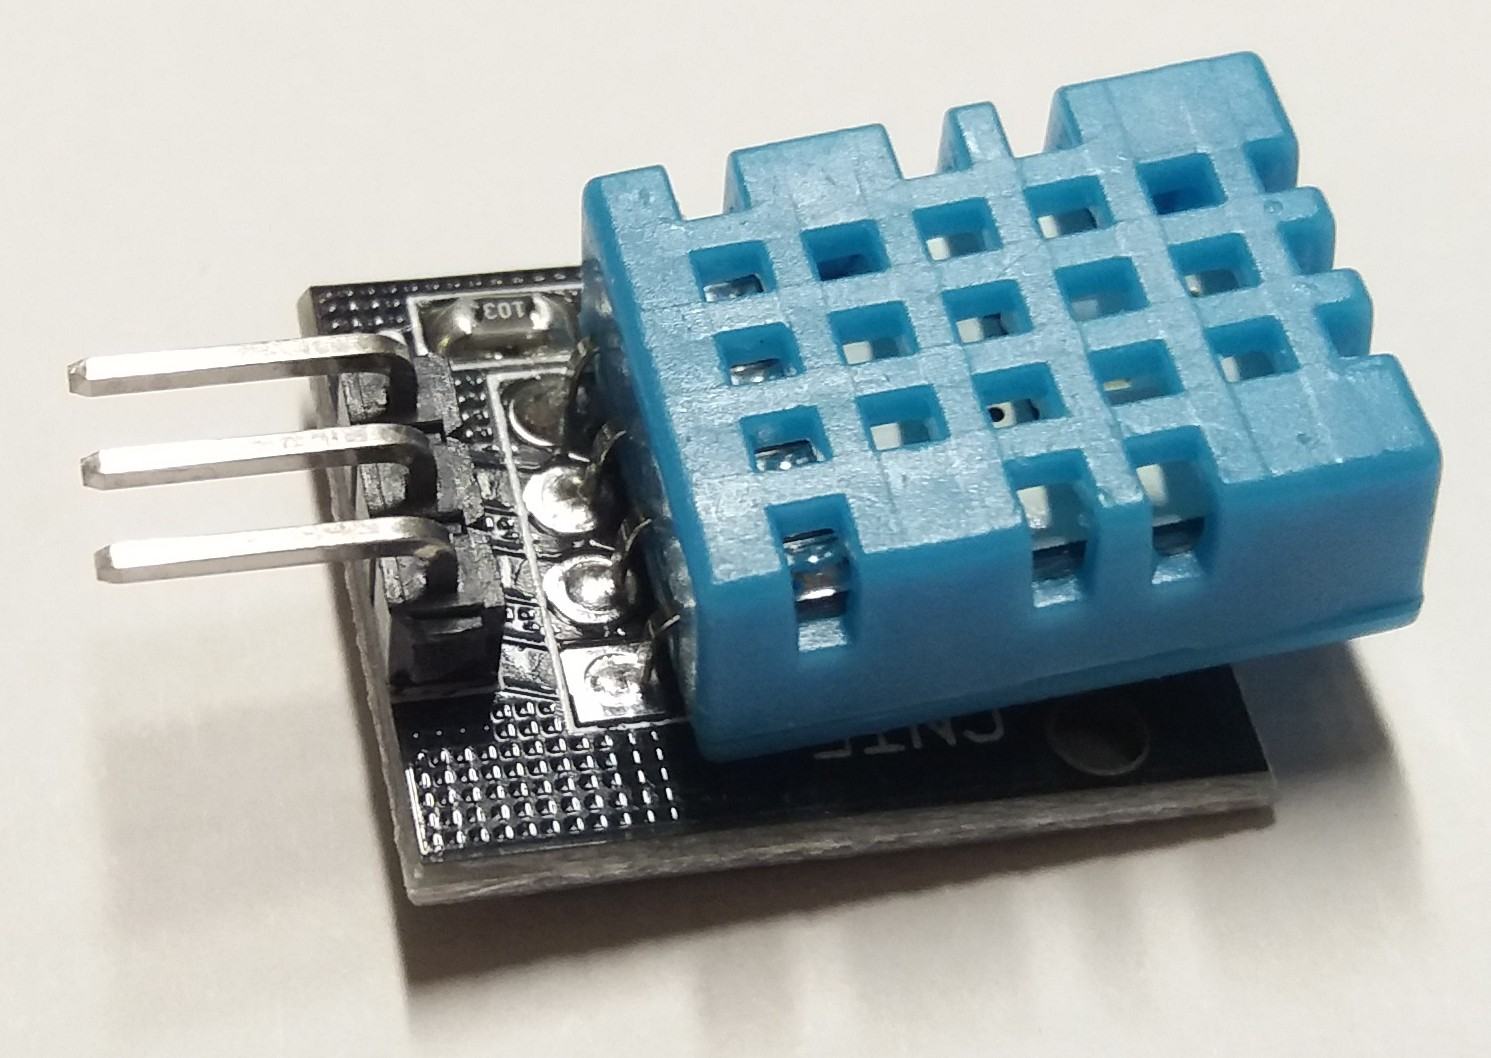
\includegraphics[width=0.84\textwidth]{./pics/dht11.jpg}
\end{minipage}
\medskip

Der DHT-11 verfügt über drei Pins - 5V und GND dienen der Stromversorgung, während das Signal zu den Messdaten über den Signalpin ausgegeben wird. Für die Temperaturmessung ist auf dem DHT-11 ein NTC verbaut.

\begin{figure}[H]
	\centering
	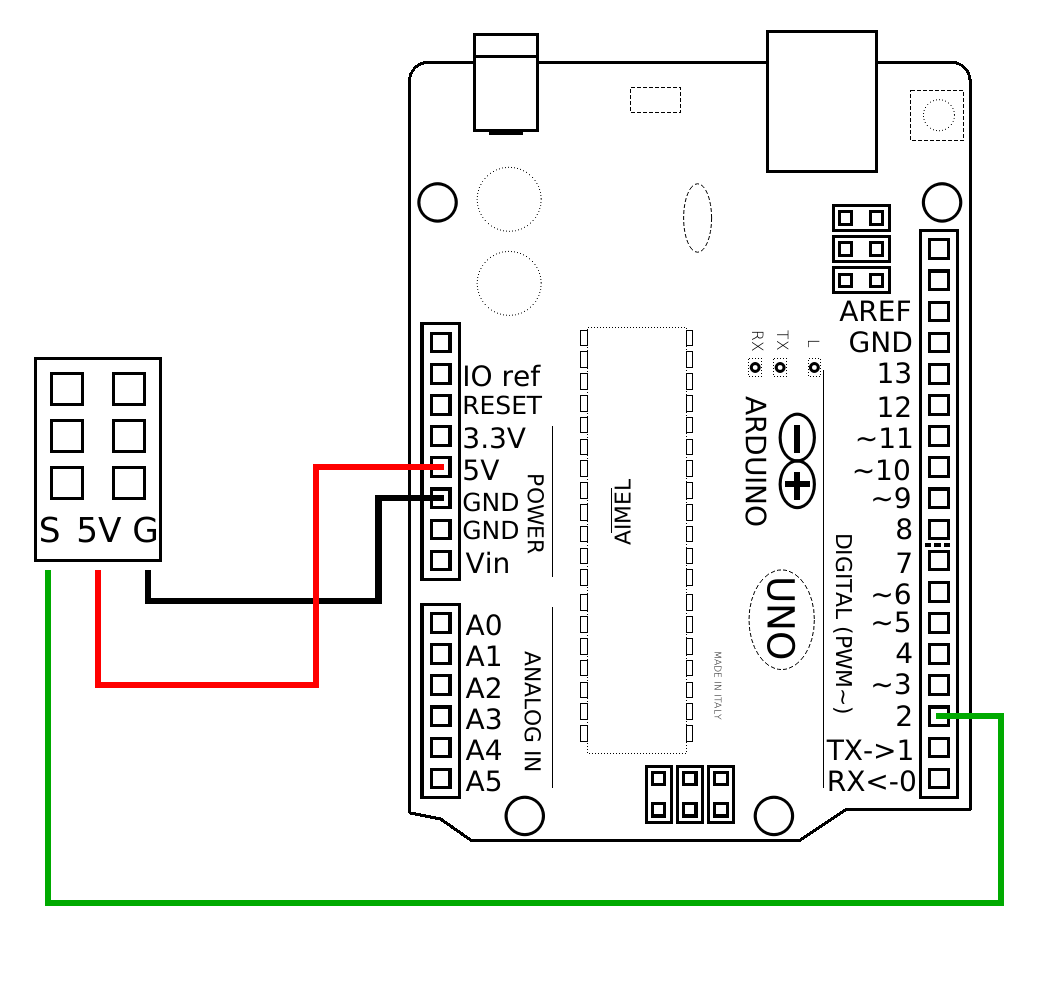
\includegraphics[width=0.4\textwidth]{./Zeichnungen/Schaltplan-DHT11.png}
\end{figure}

\vspace{-\baselineskip}
\begin{wrapfigure}{r}{0.35\textwidth}
	\centering
	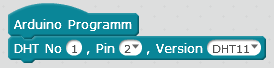
\includegraphics[width=0.35\textwidth]{./pics/dht-auslesen.png}
\end{wrapfigure}
Das Auslesen des Signalpins ist einfach, weil es von einer Erweiterung erledigt wird, die die Analyse des Signals übernimmt und Befehle bereitstellt, mit denen sich direkt auf die Temperatur und die Luftfeuchtigkeit zugreifen lässt. Zum Einbinden der Erweiterung wählt man \button{Extensions} $\rightarrow$ \button{Extensions verwalten} und sucht nach \enquote{dht}. Es sollte die Erweiterung \enquote{DHT Extensions} installiert werden. Diese bietet neben zwei Befehlen zum Auslesen von Temperatur und Luftfeuchtigkeit einen Befehl zum Initialisieren des DHT-Objekts im Programm. Dieser Befehl muss direkt nach dem Programmstart eingefügt werden.

\bigskip
\begin{projekt}[Wetterstation]\label{proj:wetterstation}
	Baue eine kleine Wetterstation, die alle zehn Minuten Temperatur und Luftfeuchtigkeit misst und auf dem seriellen Monitor ausgibt.
\end{projekt}
% Wetterstation
%Badezimmerlüfter

\begin{recherche}{Wie wird die Luftfeuchtigkeit gemessen?}
	Mit dem DHT-11 lässt sich die relative Luftfeuchtigkeit bestimmen. Recherchiere, was darunter zu verstehen ist, und wie diese durch ein elektrisches Bauteil gemessen wird.
\end{recherche}


